% FILE: sentiment.tex  Version 0.01
% AUTHOR: Uladzimir Sidarenka

% This is a modified version of the file main.tex developed by the
% University Duisburg-Essen, Duisburg, AG Prof. Dr. Günter Törner
% Verena Gondek, Andy Braune, Henning Kerstan Fachbereich Mathematik
% Lotharstr. 65., 47057 Duisburg entstanden im Rahmen des
% DFG-Projektes DissOnlineTutor in Zusammenarbeit mit der
% Humboldt-Universitaet zu Berlin AG Elektronisches Publizieren Joanna
% Rycko und der DNB - Deutsche Nationalbibliothek

\section{Sentiment Corpus}\label{sec:snt:corpus}

A crucial prerequisite for proving or disproving any hypotheses in
computational liguistics is the existence of sufficiently big manually
labeled data for the targeted domain, on which these conjectures could
be tested.  Since there was no corresponding manually annotated
sentiment corpus for German Twitter that we were aware of at the time
of writing this thesis, we had to create our own dataset, which we
will introduce in this section.

We begin our introduction by describing the selection criteria and
tracking procedure we used initially to collect the raw data for our
``tweebank''.  After detailing the annotation scheme and presenting
the utilized annotation tool, we turn to an extensive analysis of the
inter-annotator agreement, which will serve as an upper bound in our
later experiments.  In Subsection \ref{subsec:snt:iaa}, we propose two
new versions of the popular $\kappa$ metric \cite{Cohen:60} -- binary
and proportional kappa -- which were specifically adjusted to the
peculiarities of our annotation task.  With these two measures, we
estimate the inter-coder reliability of the annotated spans of
subjective opinions, their targets, and sources, also checking whether
the annotators agreed on the polarity and intensity of sentiments and
polar terms, once they agreed on their boundaries.  Finally, with
statistical means, we investigate the correlations between the
selection criteria we applied initially and the number of annotated
elements and disagreements of our experts in the corpus.  That way, we
hope to get a better understanding of which linguistic and
extra-linguistic factors might significantly influence the
distribution of sentiments, and which ones might notably exacerbate
their analysis.

\subsection{Data Collection}

A common question that typically arises when creating a new dataset is
that of the selection criteria to use in order to collect the initial
corpus data.  While, for low-level NLP tasks, such as part-of-speech
tagging or syntactic parsing, it typically suffices to define the
language domain to sample from (since the phenomena of interest are
usually frequent and uniformly spread), for semantically demanding
tasks with many diverse ways of expressions, one also has to pay
attention to various in-domain factors as they might considerably
affect the desired distribution, making the resulting corpus either
utterly sparse or excessively biased.

To minimize both of these risks -- scarceness and bias -- when
preparing our data, we decided to use a compromise approach by
gathering one part of the new corpus from tweets which were a priori
more likely to contain sentiments and sampling the rest of the
microblogs from a big collection of messages uniformly at random.  By
doing so, we hoped to increase the recall with the former strategy,
while mitigating the introduced bias with the latter method.

As criteria which could help us find more opinionated microblogs, we
considered the topic and form of tweets.  Our motivation was that some
subjects, such as political or social issues, by themselves could
incite people to be more subjective in their judgements.  Therefore,
including such topics in our corpus would automatically increase the
coverage of sentiments.  On the other hand, opinions also need to be
expressed by some linguistic means, consequently, the mere form of a
message might also suggest whether it is likely to be emotional or
not.

Since we started creating the corpus in the spring 2013, obvious
choices of subjectively rich topics to us were the \emph{papal
  conclave}, which took place in March of that year, and the
\emph{federal elections in Germany}, which were to be held in autumn.
Because both of these events implied some sort of voting, we decided
to include \emph{general discussions of political issues} as another
topic in our dataset in order to counterbalance the election
specifics.  Finally, to obey the second objective, i.e., to keep the
corpus bias low, we considered \emph{casual everyday conversations}
without any pre-defined subjects as the last source of the new data.

In order to collect tweets for the first three topics, we created
extensive keyword lists (with several dozens entries each) for each of
these subjects.  Based on these lists, we subsequently were tracking
microblogs between March and September 2013 using the public Twitter
API.\footnote{\url{https://pypi.python.org/pypi/tweetstream}}
Afterwards, the set of tweets pertaining to the federal elections was
enriched with additional messages, which we obtained from the
University of M\"unster, who were concurrently working on related
problems within the joint FMER project ``Discourse Analysis of Social
Media''.  For sampling the fourth topic, we used the German Twitter
snapshot of \citet{Scheffler:14}, which comprised all German
microblogs posted in April 2013.

%% For our work, the in-domain factors to consider were the topics and
%% the form of tweets.  Since we wanted our corpus to be as
%% representative as possible, we had to make sure that the topics we
%% choose for sampling lend themselves as fruitful opinion sources.  At
%% the same time, we did not want automatically generated ad and news
%% tweets to spoil our data and also introduced additional formal
%% criteria (described below) that the tweets had to satisfy in order to
%% be chosen.  But then again, applying these restriction might make the
%% dataset excessively biased, so we did allow for a certain proportion
%% of tweets being selected even if they did not conform to our
%% constraints.

%% Politics: 59,531 messages, keywords: Altmaier, Wowereit, Minister,
%% Bundeskanzleramt, Schwarz-Gelb

%% Papst: 51,579 messages, keywords: papst, pabst, konklave, Vatikan
%% General Tweets: 51,579 messages, keywords: papst, pabst, konklave, Vatikan

%% Federal Elections: 3,131,315 messages, keywords:

%% General: 24,179,871 messages, keywords:

This tracking procedure gave us a total of 27.4 M messages with the
M\"unster corpus and Scheffler's collection being by far the most
prolific sources of the data.  In the next step, we separated all
tweets of the same topic into three groups based on the following
formal features:
\begin{itemize}
\item We put messages that contained at least one polar term from the
  sentiment lexicon SentiWS \cite{Remus:10} into the first group;
\item Microblogs which did not satisfy the first criterion but
  featured at least one emoticon or exclamation mark were put into the
  second set;
\item Finally, all remaining tweets were allocated to the third formal
  category of their respective topic.
\end{itemize}
With this split, we, again, hoped to increase the recall of sentiments
by separately analyzing messages with already known polar terms, which
were indirectly more likely to contain subjective opinions as well.

In order to find such terms, we considered three major German polarity
lists: SentiWS \cite{Remus:10}, German Polarity Clues
\cite{Waltinger:10}, and the Zurich Sentiment Lexicon of
\citet{Clematide:10}, choosing in the end the first one due to its
moderate size, acceptably high precision, and the availability of
inflection forms of its entries.

Since no polar lexicon, however, is guaranteed to provide for the full
coverage of opinionated expressions and, moreover, because Twitter
users are renowned for their creativity in instantly inventing new
language forms \cite{Eisenstein:13}, we also applied a bail-out
approach by separately collecting messages which did not have any
lexicon terms but did contain a smiley or exclamation point.  Our
assumption was that either these elements alone would suffice to
express subjective opinions or that they would reinforce the meaning
of some accidentally missed polar words.

Finally, as we did not make any hypotheses about the distribution of
sentiments in the rest of the tweets, we allocated all remaining
microblogs to the same group, hoping that a uniform sampling would
provide us with further positive and negative opinion examples.

A detailed breakdown of the resulting distribution of messages across
the four topics and their formal groups is given in
Table~\ref{snt:tbl:corp:topic-bins}:
\begin{table}[hbt!]\small
  \begin{tabular}{|l|*{5}{>{\centering\arraybackslash}p{0.12\textwidth}|}}
    \hline

    \cellcolor{cellcolor}& \multicolumn{4}{c|}{{\cellcolor{cellcolor}}
      Formal Criterion} &
    \cellcolor{cellcolor}\\\hhline{|>{\arrayrulecolor{cellcolor}}-*{4}{>{\arrayrulecolor{black}}|-}|>{\arrayrulecolor{cellcolor}}-|}\arrayrulecolor{black}

    \multirow{-2}{0.2\columnwidth}{\centering\bfseries\cellcolor{cellcolor}
      Topic} & {\cellcolor{cellcolor}} Polar Terms
    &{\cellcolor{cellcolor}} Emoticons and Exclamations
    &{\cellcolor{cellcolor}} Remaining tweets &
             {\cellcolor{cellcolor}}Total
             &\multirow{-2}{0.12\textwidth}{\centering\cellcolor{cellcolor}
               Sample\\ Tracking\\ Keywords}\\\hline

    Federal Elections & 537,083 (22.38\%) & 50,567 (2.1\%) & 1,811,742
    (75.5\%) & 2,399,392 & \tiny\emph{Abgeordnete}
    (\emph{representative}), \emph{Bundesregierung}
    (\emph{federal government})\\\hline

    Papal Conclave & 7,859 (15.11\%) & 1,260 (2.42\%) & 42,879
    (82.46\%) & 51,998 & \tiny\emph{Papst} (\emph{pope}), \emph{Pabst} (\emph{pobe})\\\hline

    Political Discussions & 10,552 (25.8\%) & 777\newline (1.9\%) & 29,555
    (72.29\%) & 40,884 &\tiny\emph{Politik} (\emph{politics}),
    \emph{Minister} (\emph{minister})\\\hline

    General Conversations & 3,201,847 (18.7\%) & 813,478 (4.7\%) &
    13,088,008 (76.5\%) & 17,103,333 & \tiny\emph{den} (\emph{the}),
    \emph{sie} (\emph{she})\\


    \hline
  \end{tabular}
  \caption{Distribution of the downloaded messages across the topics
    and formal groups.\newline (percentage numbers are given with
    respect to the total number of tweets pertaining the
    topic)\label{snt:tbl:corp:topic-bins}}
\end{table}

As can be seen from the table, the vast majority of the tweets in each
topic fall into the third category, i.e., the one where neither polar
terms no common emoticons are present.  The average expected
proportion $\mu$ of such tweets is 76,69\%, and the standard deviation
$\sigma$ from this proportion comes to 4.25\%.  The second biggest
set, whose $\mu$ is equal to 20.5\% and $\sigma$ amounts to $4.62\%$,
is that of microblogs containing emotional terms.  Finally, the group
comprising messages with smileys but supposedly no polar terms is the
smallest one for each topic.  The expected proportion of this group
only attains $2.78\%$, deviating by $1.3\%$.

Furthermore, as one also can observe, the relative proportions of the
formal tweet groups for the federal elections and political
discussions are approximately the same, while general conversations
are apparently more biased towards containing polar terms, whereas
tweets about the papal conclave, on the contrary, are rather supposed
to be objectve.  We will check later in Subsection
\ref{subsec:snt:iaa} whether the distribution of the annotated
sentiments correlates with this proportional split of groups and
topics.

Eventually, to generate our final corpus, we randomly chose 666
messages from each of the three formal groups of each of the four
subjects, getting a total of 7,992 microblogs: $666\text{ tweets}
\times 4\text{ topics} \times 3\text{ formal criteria}$.  Although
this quota sampling admittedly violates the uniformity principle,
which states that the analyzed examples have to be chosen uniformly
from the whole population, we justify this with the wish to increase
the recall of the phenomena in question and point out to the
possibility of restoring the original distribution parameters by
multiplying the resulting statistics with the proportion coefficients
from Table~\ref{snt:tbl:corp:topic-bins}.

\subsection{Annotation Scheme}\label{subsec:snt:ascheme}
In the next step after collecting the raw data, we defined an
annotation scheme for our corpus. Since our goal was to get a
maximally full coverage of all sentiment-relevant aspects, we devised
an extensive list of elements that had to be annotated by the experts.
This list included the following annotation entities:

\begin{itemize}
\item
  \textbf{sentiments}, which we specified as polar subjective
  evaluative opinions about people, subjects, or events.  Three
  important constraints that a potential subjective statement had to
  satisfy in order to be considered as a sentiment according to our
  definition were:
  \begin{inparaenum}[\itshape a\upshape)]
  \item its \textit{polarity}, i.e., the statement in question had to
    reflect either positive or negative attitude;
  \item \textit{subjectivity}, i.e., the expressed opinion had to be
    a personal attitude, not verifiable by any objective means; and,
    finally,
  \item this judgment had to be \textit{evaluative}, i.e., it had to
    refer to some clearly discernable target from its surrounding
    context.
  \end{inparaenum}

  Following \citet{Jindal:06a,Jindal:06b}, we explicitly addressed the
  cases of comparisons, considering them as a special type of
  sentiment \emph{polarity} in addition to regular positive and
  negative opinions and providing a corresponding value for this
  attribute.\footnote{The complete list of the annotation elements and
    their attributes can be found in the original annotation
    guidelines provided in Appendix~\ref{chap:apdx:sent}.}  Further
  attributes associated with the sentiment elements included
  \emph{intensity} with the values ranging over weak, medium, and
  strong, and the boolean attribute \emph{sarcasm}, with which our
  annotators marked opinions whose actual polarity was the opposite of
  the apparent form, e.g. ``Mein j\"ungerer Bruder ist in der
  Pr\"ufung durchgefallen.  Klasse!''  (\textit{My younger brother has
    failed his exam.  Well done!});

\item another annotation element, which was closely related to
  sentiments, were \textbf{targets}, which we defined as objects or
  events being evaluated by sentiment expressions.  Since comparative
  opinions a priori presuposed the existence of at least two targets,
  one of which was preferred over the others, we introduced a special
  attribute \emph{preferred} for targets which were given preference
  in a comparison.  Furthermore, since some of the targets could be
  expressed by pronouns, and because coreference resolution might play
  an important role for mining opinions \cite{Stoyanov:06,Ding:10}
\end{itemize}


\subsubsection{Boundaries} \texttt{sentiment} markables should
encompass both the object being evaluated (the target) and the actual
phrase phragment which expresses the evaluation (typically an
emo-expression, if it exists).  After determining these two elements,
you should put the \texttt{sentiment} tags around the \emph{minimal
  complete syntactic or discourse-level unit in which both target and
  evaluation expression appear together}.

In Example \ref{exmp:book}, for instance, the evaluated object is
\textit{Buch} (\textit{book}), the evaluative expression is
\textit{langweiliges} (\textit{boring}), and the minimal syntactic unit which
simultaneously covers both of these elements is the noun phrase \textit{ein
  langweiliges Buch} (\textit{a boring book}).  We therefore put
\texttt{sentiment} tags around this noun phrase but do not put anything else
inside them.
\begin{example}
  Auf dem Tisch lag \sentiment{ein langweiliges Buch}.

  (There was \sentiment{a boring book} on the table.)\label{exmp:book}
\end{example}
Sentiments are not restricted to just noun phrases, they can also be
expressed by complete clauses or even multiple sentences
(i.e. discourse-level units).  The main point is that a
\texttt{sentiment} span has to be \emph{complete}, i.e. it should
capture the common syntactic or discourse-level ancestor element of
both evaluation and target and also include all other decendants of
that common ancestor.  Furthermore, a \texttt{sentiment} markable has
to be \emph{minimal}, i.e. it should only cover the lowest possible
ancestor element of evaluation and target but should not include
parents or siblings of this ancestor.

Example \ref{exmp:petterson} shows how a sentiment relation can be
expressed by a clause:
\begin{example}
  Wir akzeptieren das, weil \sentiment{wir alle ein bisschen in
    Petterson verliebt sind}.

  (We accept this because \sentiment{we all are a little bit in love
    with Petterson}.)\label{exmp:petterson}
\end{example}
\noindent In this sentence, the evaluative statement is made about
\textit{Petterson} who acts as sentiment's target.  The author says
that they all \textit{in ihn verliebt sind} (\textit{are in love with
  him}) which is her subjective evaluative opinion.  Both target and
evaluative expression appear together in one verb phrase with the head
verb \textit{sein} (\textit{to be}).  So, we mark this complete verb
phrase including its grammatical subject \textit{wir} (\textit{we})
which is the syntactic descendant of the head verb.

%%%%%%%%%%%%%%%%%%%%%%%%%%%%%%%%%%%%%%%%%%%%%%%%%%%%%%%%%%%%%%%%%%%%%%%%%%%%%%%%%%%%%%%%%%
\subsection{target}
\noindent\textbf{Definition.} \emph{Targets} are objects or events
that are being evaluated by a sentiment expression.

\noindent{} Because sentiments are required to be evaluative, there
MUST always be at least one target for each sentiment relation.
Conversely, if there is no annotated sentiment, we do not annotate
targets.

Occasionally, a target may be elided (\emph{Ist gut.} / \emph{Is
  good.})  and thus is not to be marked.  However, for the reader of
the tweet it must be possible to interpret the elision, i.e., to
recover the missing constituent, in order for a sentiment to be
present.

\noindent\textbf{Example.} An example of a sentiment target is given in
Sentence \ref{exmp:target}:
\begin{example}
Mein Bruder ist nicht begeistert von \target{dem neuen Call of Duty}.

(My brother is not impressed by \target{the new Call of
  Duty}.)\label{exmp:target}
\end{example}
\noindent In this sentence, the author is telling us about the subjective
opinion of her brother regarding the new version of a computer game.  This new
computer game is the object of the evaluation and we annotate it as
\texttt{target}.

\noindent\textbf{Boundaries.} Similar to \texttt{sentiment}s, you should put
the \texttt{target} tags around the minimal complete syntactic or
discourse-level units which denote the objects or events being evaluated.
These are usually noun phrases (e.g. \textit{Mir wird's schlecht, wenn ich
  \target{diese Werbung} im Fernsehen sehe} (\textit{I feel sick when I see
  this \target{ad} on TV})) or clauses (e.g. \textit{Ich hasse wenn
  \target{Voldemort mein Shampoo benutzt}.} (\textit{I hate when
  \target{Voldemort is using my shampoo}})).

In case a target is an anaphoric expression (a pronoun) and its
antecdent (a full NP) is present in the same tweet (be it within or
outside of the sentiment span), both are being annotated and linked
with an \emph{anaph-ref} relation (see Table \ref{tbl:target}).

Occasionally, a Twitter hashtag or @-mention may serve as a target.
Then they are marked as usual, without adding a specific attribute.

If a sentiment has multiple targets, you should mark each one of them
separately (cf. Example \ref{exmp:trg-conj}).
\begin{example}
  Meiner Mutter haben \target{Nelken} und \target{Dahlien} immer gefallen.

  (My mother has always liked \target{carnations} and
  \target{dahlias}.)\label{exmp:trg-conj}
\end{example}

Similar, in comparisons, you should also annotate each compared object
separately.  Additionally, for the object which is being dispreferred,
you should also set the value of the \texttt{preferred} attribute to
\texttt{false} (cf. Example \ref{exmp:trg-comp}).
\begin{example}
  Ich mag \target[preferred=true]{Domino-Eis} mehr als
  \target[preferred=false]{Magnum}.

  (I like \target[preferred=true]{Domino ice cream} more than
  \target[preferred=false]{Magnum}.)\label{exmp:trg-comp}
\end{example}

\noindent\textbf{Attributes.} Further possible attributes of \texttt{target}s
are shown in Table \ref{tbl:target}.
\begin{center}
  \begin{table}[h]
    \caption{Attributes and values of \texttt{target}s.}
    \begin{tabular}{|l|c|p{0.94\clmnwidth}|}\hline
      Attribute & Value & Value's Meaning\\\hline

      & \textit{true} (default) & in comparisons, this value means that
      the respective target is being considered better than another
      compared object, e.g. \textit{\emph{Die neue Frisur} passt ihr
        garantiert besser als die alte (\emph{The new hairstyle} suits
        her definitely better than the old one)};\\\cline{2-3}

      \multirow{-2}{*}{preferred} & \textit{false} & in comparisons,
      this value marks the target element which is being considered
      worse than its counterpart, e.g. \textit{Die zweite Saison von
        Breaking Bad war viel spannender als \emph{die dritte} (The
        second season of Breaking Bad was much more exciting than
        \emph{the third one})};\\\hline

      sentiment-ref & \textit{$\longrightarrow$\newline(directed
        edge)} & directed edge pointing from \texttt{target} to its
      respective \texttt{sentiment}.  You need to draw this edge in
      two cases:
      \begin{itemize}
      \item when the \texttt{target} is located at intersection of two
        different \texttt{sentiment}s (in this case, you should draw
        an edge from \texttt{target} to \texttt{sentiment}, which this
        \texttt{target} actually belongs to),

      \item when the target of an opinion is expressed outside the
        \texttt{sentiment} span;
      \end{itemize}\\\hline

      anaph-ref & \textit{$\longrightarrow$\newline(directed edge)} &
      directed edge pointing from \texttt{target} expressed by a
      pronoun or pronominal adverb to its respective non-pronominal
      antecedent (in order to draw this edge, you also need to mark
      the antecedent as \texttt{target})\\\hline
    \end{tabular}
    \label{tbl:target}
  \end{table}
\end{center}

%%%%%%%%%%%%%%%%%%%%%%%%%%%%%%%%%%%%%%%%%%%%%%%%%%%%%%%%%%%%%%%%%%
%% Source
\subsection{source}
\noindent\textbf{Definition.} Sentiment \emph{sources} are immediate author(s)
or holder(s) of evaluative opinions.  These are typically writers of the
messages or persons or institutions whose opinion is being cited.

If sentiment's source of is not explicitly mentioned in the message,
we assume it to be the author of the tweet. You need not annotate
anything as \texttt{source} in this case.

In parallel with targets, sources are only annotated when a sentiment
is present. (E.g., if a tweet contains a quotation with an explicit
source, but there is no sentiment, than the source is not annotated.)

\noindent\textbf{Example.} An example of an explicit sentiment source
is the pronoun \textit{Sie} (\textit{she}) in Example
\ref{exmp:source}.
\begin{example}
  \source{Sie} mag die neue Farbe nicht

  (\source{She} doesn't like the new color)\label{exmp:source}
\end{example}

Note that in case of citations you should only mark the immediate
person or the institution whose original opinion is being cited, but
you should not mark the citing person as a \texttt{source}
(cf. Example \ref{exmp:source-citation}).
\begin{example}
  Laut Staatsanwalt soll die \source{Angeklagte} sich missbilligend \"uber
  ihren Vorgesetzten ge\"au\ss{}ert haben.

  (According to the attorney, the \source{defendant} had made
  disapproving remarks about her boss.)\label{exmp:source-citation}
\end{example}

\noindent\textbf{Boundaries.} For determining the boundaries of
\texttt{source}s, you should proceed in similar fashion as we did for
\texttt{target}s and \texttt{sentiment}s and only mark complete
minimal syntactic units.  Sources are most commonly expressed by noun
phrases.  And, similar to \texttt{target}s, if the source of a
sentiment is expressed by multiple separate noun phrases, you should
mark each of them separately (cf. Example \ref{exmp:source2}).

\begin{example}
  \source{Ihr} und \source{ihrer Mutter} gef\"allt die neue Farbe
  nicht.\\ (Neither \source{she} and \source{her mother} likes the new
  color)\label{exmp:source2}
\end{example}

\noindent\textbf{Attributes.} The attributes of the \texttt{source}
tag are listed in Table \ref{tbl:source}.  They are fully identical to
the attributes of the \texttt{target} markables.
\begin{center}
  \begin{table}[h]
    \caption{Attributes and values of \texttt{source}s.}
    \begin{tabular}{|l|c|p{0.935\clmnwidth}|}\hline
      Attribute & Value & Value's Meaning\\\hline

      sentiment-ref & \textit{$\longrightarrow$\newline(directed
        edge)} & cf. Table \ref{tbl:target}\\\hline

      anaph-ref & \textit{$\longrightarrow$\newline(directed edge)} &
      cf. Table \ref{tbl:target}\\\hline
    \end{tabular}\label{tbl:source}
  \end{table}
\end{center}

%%%%%%%%%%%%%%%%%%%%%%%%%%%%%%%%%%%%%%%%%%%%%%%%%%%%%%%%%%%%%%%%%%
%% Emo-expression
\subsection{emo-expression}
\noindent\textbf{Definition.} \emph{Emo-expressions} are lexical items
(i.e., words or idioms) that have a clearly distinguishable polar
subjective meaning.

\noindent\textbf{Example.} An example of an emo-expression is the word
\textit{ekelhaft} (\textit{disgusting}) in Example
\ref{exmp:emo-expr1}.
\begin{example}
  Beim Aufr\"aumen des Zimmers haben wir einen
  \emoexpression{ekelhaften} Teller mit verschimmeltem Essen unter dem
  Bett gefunden.

  (When we cleaned the room, we found a \emoexpression{disgusting}
  plate with moldy food under the bed.)\label{exmp:emo-expr1}
\end{example}
\noindent{} This term is unequivocally polar, since it expresses a
negative attitude towards its target, and subjective, since it stands
for a personal perception of the author.

A notable difference between \texttt{emo-expression}s on the one hand
and \texttt{source}s and \texttt{target}s on the other hand is that
\texttt{emo-ex\-pre\-ssion}s should always be annotated in text no
matter whether a target-oriented sentiment exists in their vicinity or
not. \texttt{source}s and \texttt{target}s, however, should only be
marked along with a \texttt{sentiment} element they pertain to.
Therefore, in a sentence like \emph{Ausgezeichnet!}
(\emph{Excellent!}), you should mark the single present word as an
\texttt{emo-expression} but should not annotate any
\texttt{sentiment}s in such cases (as the target of this expression is
unclear).

Another distinguishing feature of \texttt{emo-expression}s is that
they should only encompass \emph{lexical} items (i.e., words or
idioms), whereas \texttt{source}s and \texttt{target}s should
typically comprise \emph{syntactic} elements (i.e., noun and verb
phrases).  In order to decide whether a given element is a lexical
item or not, you should think about whether this element could appear
as a separate entry in a defining or idiomatic dictionary.  In case it
can, the language unit under scrutiny is a lexical element, otherwise
it is a free noun or verb phrase which should not be regarded as an
\texttt{emo-expression}.

An example of a lexical item is the word \emph{cooler} (\emph{cool})
in the sentence below:
\begin{example}
  Das war ein echt \emoexpression{cooler} Film.

  (This was a really \emoexpression{cool} movie.)
\end{example}
\noindent Since the lemma of this adjective might appear as a lexicon
entry, and its meaning is definitely positive and subjective, this
word should be annotated as an \texttt{emo-expression}.  It is,
however, unlikely that the complete noun phrase \emph{ein cooler Film}
(\emph{a cool movie}) would be included into a defining dictionary,
therefore, one should not consider this whole phrase as an
\texttt{emo-expression} instance.

In rare cases, however, some ad hoc phrases might appear like lexical
items but be too rare to be included into a lexicon.  An example of
such phrase is provided below:
\begin{example}
Norwegen erinnert an \textrm{die fr\"uhe Ursula von der Leyen}.

(Norway reminds one of \textrm{early Ursula von der Leyen}.)
\end{example}
\noindent In this sentence, the phrase \emph{die fr\"uhe Ursula von
  der Leyen} (\emph{early Ursula von der Leyen}) is a metaphoric term
which was created spontaneously for this particular sentence only.
Nevertheless, we can replace this term with an almost equivalent
lexicon synonym \emph{Einzelg\"anger} (\emph{loner}).  In such cases,
when we can provide a dictionary equivalent for an ad hoc term, we can
also consider the ad hoc phrase as an \texttt{emo-expression}, but
this should be regarded as an exception rather than regularity.

Another difficulty when annotating \texttt{emo-expression}s might
arise from the fact that many words and idioms are ambiguous and can
have several different lexical meanings, but only some of these
meanings might be polar and subjective.  In these cases, you should
only mark a lexical item as an \texttt{emo-expression} if its actual
sense in the given context is polar.  If the active meaning of the
lexeme is objective, you must not annotate it
(cf. Example~\ref{exmp:emo-expression-jewel}).
\begin{example}
  Dieser Wein ist ein echtes \emoexpression{Juwel} in meiner
  Kollektion.

  (This wine is a real \emoexpression{jewel} in my collection.)

  Koh-i-Noor ist das teuerste Juwel heutzutage.

  (Koh-i-Noor is the most expensive jewel nowadays.)\label{exmp:emo-expression-jewel}
\end{example}
\noindent{}In the above example, the meaning of the word
\textit{Juwel} (\textit{jewel}) is metaphoric and subjective in the
first sentence but literal and objective in the second.  So you should
only annotate this word as an \texttt{emo-expression} in the former
case but not mark it as such it in the latter.

Finally, it might be difficult to decide whether a polar term is
subjective or not.  Prominent examples of such borderline cases are
the so-called subjective facts, e.g., \emph{Tod} (\emph{death}),
\emph{Krankheit} (\emph{disease}), \emph{Bombe} (\emph{bomb}),
\emph{w\"ahlen} (\emph{elect}) etc., which some people perceive as
subjective expressions while others regard them as objective facts.
For such cases, we have introduced a special attribute
\texttt{subjective\_fact}, which you can set to \texttt{true} when you
encounter such expressions and think that they also belong to the
\texttt{emo-expression} class.

To summarize, when annotating emotional expressions in corpus, you
should proceed as follows:
\begin{enumerate}
  \item determine an exact word or phrase which, in your opinion,
    might have a polar lexical meaning;
  \item decide whether this word or idiom can appear as a separate
    entry in a monolingual dicionary or lexicon or not;
  \item if it can, decide which lexical meanings in general this
    phrase might have and which of them are polar;
  \item look whether the currently active meaning of this term in the
    given context is one of the polar senses;
  \item if it is, annotate the given term as an
    \texttt{emo-expression} and decide whether it is subjective or
    not;
  \item in the latter case, set the attribute \texttt{subjective\_fact}
    of the newly created \texttt{emo-expression} to the value
    \texttt{true}.
\end{enumerate}

\noindent\textbf{Boundaries.} \texttt{emo-expression}s are typically
expressed by:
\begin{itemize}
  \item nouns, e.g. \textit{Held (hero)}, \textit{Ideal (ideal)},
    \textit{Betr\"uger (fraudster)} etc.;

  \item adjectives or adverbs, e.g. \textit{sch\"on (nice)},
    \textit{zuverl\"assig (reliably)}, \textit{hinterh\"altig
      (devious)}, \textit{heimt\"uckisch (insidiously)} etc.;

  \item verbs, e.g. \textit{lieben (to love)}, \textit{bewundern (to
    admire)}, \textit{hassen (to hate)} etc.;

  \item idioms, e.g. \textit{auf die Nerven gehen (to get on one's
    nerves)} etc.;

  \item smileys, e.g. :), :-(, \smiley{}, \frownie{} etc.
\end{itemize}
If an \texttt{emo-expression} is formed by an idiomatic phrase, you should
always annotate the complete idiom.  For verbs which take on an evaluative
sense only if used with certain prepositions (e.g. \textit{to go for sth.} in
the sense of \textit{to like}), you should annotate both the verb and the
preposition as a single markable (please refer to the \texttt{MMAX} manual to
see how to annotate discontinuous spans).

Occasionally, a Twitter hashtag may serve as an emo-expression
(\emph{\#excellent}).  They are marked as usual, without adding a
specific attribute.

\noindent\textbf{Attributes.} When determining the value of the
\texttt{polarity} attribute of an \texttt{emo-expression}, you should
disregard any possible contextual modifiers like intensifiers or
negations and set the value of this attribute to the lexical (or also
called \emph{prior}) polarity of the phrase (the one it would have
without any negations and other modifiers) (cf. Example
\ref{exmp:emo-expression-polarity}).
\begin{example}
Es war keine \emoexpression[polarity=positive]{gute} Idee.

(It was not a \emoexpression[polarity=positive]{good} idea.)\label{exmp:emo-expression-polarity}
\end{example}

Also, when determining the value of the \texttt{polarity} attribute of
an \texttt{emo-expression}, you should analyze its polarity from the
perspective of the subject or event which is being evaluated (in case
when such subject is present in the context).  This means that in
cases like \textit{Ich vermisse meine Freundin} (\textit{I miss my
  girlfriend}), the polarity of the emo-expression \textit{vermissen}
(\textit{to miss}) is still positive because the author evidently has
a positive attitude to the girlfriend even if he experiences sadness
because of her absence.

Further attributes of \texttt{emo-expression}s include
\texttt{intensity}, \texttt{sarcasm}, \texttt{subjective\_fact}, and
\texttt{sentiment-ref}.  Possible values and descriptions of these
attributes are summarized in Table \ref{tbl:emo-expression}.
\begin{center}
  \begin{table}[ht]
    \caption{Attributes and values of \texttt{emo-expression}s.}
    \begin{tabular}{|l|c|p{0.935\clmnwidth}|}\hline
      Attribute & Value & Value's Meaning\\\hline
      %%%%%%%%%%%%%%%%%%%

      & \textit{positive} & emotional expression has a positive
      evaluative meaning, e.g. \textit{gut (good), verhimmeln (to
        ensky), Prachtkerl (corker)} etc.\\\cline{2-3}

      \multirow{-2}{*}{polarity} & \textit{negative\newline(default)}
      & emotional expression has a negative evaluative meaning towards
      its target, e.g. \textit{versauen (to botch up), rotzig
        (snotty), Dreckskerl (scum)} etc.\\\hline

      %%%%%%%%%%%%%%%%%%%

      & \textit{weak} & emo-expression has a weak evaluative sense,
      e.g. \textit{solala (so-so), nullachtf\"unfzehn (vanilla),
        durchschnittlich (mediocre)} etc.\\\cline{2-3}

      & \textit{medium\newline(default)} & emo-expression has middle
      stylistic expressivity, e.g. \textit{gut (good), schlecht (bad),
        robust (tough)} etc.\\\cline{2-3}

      \multirow{-3}{*}{intensity} & \textit{strong} & emo-expression
      expresses a very strong positive or negative evaluation,
      e.g. \textit{allerbeste (bettermost), zum Kotzen (to make one
        puke), Kacke (shit)} etc.\\\hline

      %%%%%%%%%%%%%%%%%%%%

      \multirow{2}{*}{sarcasm} & \textit{true} & emo-expression is
      derisive, i.e. its actual polarity is the opposite of its
      apparent form. (This means that an apparent praise which appears
      in text is in fact meant as a rebuke and vice versa. The actual
      sense, however, can only be inferred on the basis of world
      knowledge or reasoning.)\\\cline{2-3}

      & \textit{false\newline(default)} & no sarcasm is present -- the
      polar attitude has its literal meaning; this is the default
      setting\\\hline

      %%%%%%%%%%%%%%%%%%%%

      \multirow{2}{*}{subjective\_fact} & \textit{true} & the
      emo-expression represents a possibly objective circumstance,
      which, however, might have a clear polar association or
      connotation, e.g., \emph{Nordkorea} (\emph{North Korea}),
      \emph{Atomtest} (\emph{atom test}), \emph{Diabetes}
      (\emph{diabetes}) etc.\\\cline{2-3}

      & \textit{false\newline(default)} & the emo-expression expresses
      a purely subjective attitude\\\hline

      %%%%%%%%%%%%%%%%%%%%

      \multirow{2}{*}{uncertain} & \textit{true} & the annotator is
      uncertain whether the given term is an emotional expression or
      not, e.g. \emph{angetrunken} (\emph{half-drunk}),
      \emph{einf\"altig} (\emph{na\"{i}ve})\\\cline{2-3}

      & \textit{false\newline(default)} & the given term unequivocally
      forms an emo-expression\\\hline

      %%%%%%%%%%%%%%%%%%%

      sentiment-ref & \textit{$\longrightarrow$\newline(directed
        edge)} & arrow pointing to the \texttt{sentiment} which this
      \texttt{emo-expression} belongs to.  You should only draw this
      edge if an \texttt{emo-expression} is located in the overlapping
      of two \texttt{sentiment} spans or outside of the
      \texttt{sentiment} span which it belongs to\\\hline
    \end{tabular}
    \label{tbl:emo-expression}
  \end{table}
\end{center}

%%%%%%%%%%%%%%%%%%%%%%%%%%%%%%%%%%%%%%%%%%%%%%%%%%%%%%%%%%%%%%%%%%
%% Intensifier
\subsection{intensifier}
\noindent\textbf{Definition.} \emph{Intensifiers} are elements which increase
the expressivity and the polar sense of an emotional expression.

\noindent\textbf{Example.} An example of an intensifier is the word
\textit{sehr} (\textit{very}) in Example \ref{exmp:intensifier}.
\begin{example}
  Wir suchen eine \intensifier{sehr} zuverl\"assige Polin als
  Haushaltshilfe.

  (We are looking for a \intensifier{very} reliable Polish woman as
  domestic help.)\label{exmp:intensifier}
\end{example}
\noindent\textbf{Boundaries.} Intensifiers are usually expressed by
adverbs or adjectives like \textit{sehr} (\textit{very}), sicherlich
(\textit{certainly}) etc., but other ways of expressing them are still
possible (cf. Example \ref{exmp:intensifier-comp}).  However, we only
regard separate lexical items as intensifiers: iterated letters, as in
gooood are not annotated, and neither are punctuation marks (such as
exclamation marks).

\begin{example}
  Dieser Junge ist stark \intensifier{wie ein Pferd}.

  (This boy is strong \intensifier{as a
    horse}.)\label{exmp:intensifier-comp}
\end{example}

\noindent\textbf{Attributes.} An \texttt{intensifier} should always
relate to some \texttt{emo-expression} and you should also always
explicitly show that relation by drawing an edge attribute from
\texttt{intensifier} to its respective \texttt{emo-expression}
markable.

Further possible attributes of \texttt{intensifier}s are shown in
Table \ref{tbl:intensifier}.
\begin{center}
  \begin{table}[htb]
    \caption{Attributes and values of \texttt{intensifier}s.}
    \begin{tabular}{|l|c|p{0.875\clmnwidth}|}\hline

      & \textit{medium (default)} & the intensifier moderately
      increases the polar sense of the emotional expression,
      e.g. \textit{ziemlich (quite), recht (fairly)} etc.\\\cline{2-3}

      \multirow{-2}{*}{degree} & \textit{strong} & the intensifier
      strongly increases the polar sense and stylistic markedness of the
      emotional expression, e.g. \textit{sehr (very), super (super),
        stark (strongly)} etc.\\\hline

      %%%%%%

      emo-expression-ref & \textit{$\longrightarrow$\newline(directed
        edge)} & a directed edge pointing from the intensifier to the
      \texttt{emo-expression} whose meaning is being intensified\\\hline
    \end{tabular}
    \label{tbl:intensifier}
  \end{table}
\end{center}

\subsection{diminisher}
\noindent\textbf{Definition.} \emph{Diminisher}s are words or phrases
that decrease the polar lexical sense of an \texttt{emo-expression}.

\noindent\textbf{Example.} In Example \ref{exmp:diminisher}, the
diminisher is expressed by the adverb \textit{weniger}
(\textit{less}).
\begin{example}
  \diminisher{Weniger} erfolgreiche Unternehmen verzichten auf externe
  Berater.\label{exmp:diminisher}

  The \diminisher{less} successful companies do not use external
  consultants.
\end{example}
\noindent\textbf{Attributes.} Similar to intensifiers, diminishers
should always relate to some emotional expression and you should also
explicitly show this relation by drawing an edge attribute.

The attributes of diminishers mainly correspond to that of
intensifiers.  The only difference concerns the \texttt{degree}
attribute which shows how strong an intensifier \emph{increases} but a
diminisher \emph{decreases} the lexical sense of an emo-expression.  A
list of possible attributes for the \texttt{diminisher}s is summarized
in Table \ref{tbl:diminisher}.
\begin{center}
  \begin{table}[hb]
    \caption{Attributes and values of \texttt{diminisher}s.}
    \begin{tabular}{|l|c|p{0.88\clmnwidth}|}\hline

      & \textit{medium (default)} & diminisher moderately decreases
      the polar sense of its respective \texttt{emo-expression},
      e.g. \textit{wenig (few), bisschen (little)} etc.\\\cline{2-3}

      \multirow{-2}{*}{degree} & \textit{strong} & diminisher strongly
      decreases the polar sense of the \texttt{emo-expression},
      e.g. \textit{kaum (hardly)} etc.\\\hline

      emo-expression-ref & \textit{$\longrightarrow$\newline(directed
        edge)} & see Table \ref{tbl:intensifier}\\\hline
    \end{tabular}
    \label{tbl:diminisher}
  \end{table}
\end{center}

\subsection{negation}
\noindent\textbf{Definition.} \emph{Negation}s are elements which turn
the polarity of an \texttt{emo-expression} to the complete opposite.

\noindent\textbf{Example.} In Example \ref{exmp:negation}, for
instance, the negative article \textit{kein} (\textit{not}) makes the
\emph{contextual} polarity of the word \textit{interessant}
(\textit{interesting}) to be negative, even though the prior polarity
of this word is unequivocally positive.
\begin{example}
Diese Geschichte war \"uberhaupt nicht \negation{interessant}!

This story was \negation{not} interesting at all!\label{exmp:negation}
\end{example}

The role and the meaning of negations are closely related to that of
diminishers.  In order to help you better differentiate between these
elements, we have listed the most obvious differences between the two
classes:
\begin{itemize}
  \item\textit{Semantic differences}.  While diminishers only decrease
    the lexical sense of an emo-expression, a part of this original
    sense still remains active (i.e. \textit{a hardly understandable
      speech} is still understandable); negations, on the contrary,
    fully deny that meaning and turn it to the complete opposite
    (\textit{a not understandable speech} is absolutely
    unintelligible);

  \item\textit{Part-of-speech differences}.  While diminishers are
    usually expressed by adjectives or adverbs, negations are
    typically represented by the negative article \textit{kein (no)},
    the negation particle \textit{nicht (not)}, or adjectives or
    verbs, e.g.  \textit{Es ist sehr zweifelhaft, dass die neue
      Version von Windows besser wird} (\textit{It is very doubtful
      that the new Windows version will be any better})

  %% \item\textit{Syntactic differences}.  While diminishers are usually
  %%   expressed by either adjectives or adverbs; negations, on the contrary,
  %%   are commonly represented by either the negative article \textit{kein
  %%   (no)} or the negation particle \textit{nicht (not)}, or even complete
  %%   clauses (\textit{Er ist nicht einverstanden, dass die neue Version von
  %%   Windows besser ist (He disagrees that the new Windows version is any
  %%   better)}).
\end{itemize}

\noindent\textbf{Attributes.} The only attribute of negations is the
mandatory edge \texttt{emo-expression-ref}.  You should draw this edge
from the \texttt{negation} to the \texttt{emo-expression} being
negated.  Like intensifiers and diminishers, negations should always
relate to at least one \texttt{emo-expression}.
\begin{center}
  \begin{table}
    \caption{Attributes and values of \texttt{negation}s.}
    \begin{tabular}{|l|c|p{0.875\clmnwidth}|}\hline
      emo-expression-ref & \textit{$\longrightarrow$\newline(directed
        edge)} & an edge from \texttt{negation} to the
      \texttt{emo-expression} being negated\\\hline
    \end{tabular}
    \label{tbl:negation}
  \end{table}
\end{center}

\begin{itemize}
  \item\textbf{emotional expressions}, which we defined as words or
    phrases that unequivocally possessed some evaluative lexical
    meaning (e.g., \emph{gut} ``good'', \emph{schlecht} ``bad'', or
    \emph{lieben} ``to love'');
  \item\textbf{intensifiers}, which were specified as elements that
    increased the expressivity or the polar sense of emotional items
    (for instance, \emph{sehr} ``very'' or
    \emph{au\ss{}ergew\"ohnlich} ``extraordinarily'');
  \item\textbf{diminishers}, which we described as lexical instances
    that decreased the polar sense of an emotional expression (for
    example, \emph{wenig} ``little'' or \emph{kaum} ``hardly'');
  \item and \textbf{negations}, which were linguistic means that
    turned the polarity of an emotional expression to the complete
    opposite.
\end{itemize}

Additionally, in order to capture the interrelationship between the
polar terms (emotional expressions in our case) and the entities they
characterized, we also introduced the following elements in our
scheme:
\begin{itemize}
  \item\textbf{targets}, which we described as objects or events that
    were evaluated by sentiment expressions;
  \item\textbf{sources}, which were immediate author(s) or holder(s)
    of evaluative opinions;
  \item and actual \textbf{sentiments}, which we specified as minimal
    complete syntactic or discourse-level units in which both target
    and evaluative expression appeared together.
\end{itemize}

\noindent{}A sample tweet annotated according to our definitions is
provided below:

{
  \renewcommand{\thesection}{\arabic{section}}
  \begin{example}

    \upshape\sentiment{\target{Diese Milliardeneinnahmen} sind selbst
      \source{Sch\"auble} \emoexpression{peinlich}}\\[0.8em]
    \noindent\sentiment{\target{\itshape{}These billions of
        revenues\upshape{}}\itshape{} are\upshape{}
      \emoexpression{\itshape{}embarrassing\upshape{}}\itshape{} even for
      \upshape{}\source{\itshape{}Sch\"auble\upshape{}}}
  \end{example}
}

Beside annotating text spans of opinion-relevant items, our experts
also specified the values of the attributes associated with these
elements. For emotional expressions and sentiments, they determined
the \emph{polarity} and \emph{intensity} of the respective judgements,
distinguishing between positive, negative, and comparative cases for
the former attribute and using a three point scale (weak, medium, and
strong) for assessing the intensity.

Furthermore, we explicitly addressed the cases of \emph{sarcasm} by
providing a separate attribute for ironically meant polar terms and
opinions.  In total, our experts were able to find 145 cases of
sarcastic sentiments, also detecting 82 examples of mocking lexical
phrases.

For diminishers and intensifiers, the annotators were also asked to
set the \emph{degree} of these elements, which showed by how much they
were changing the intensity of their respective emotional expressions.
Finally, in cases when sources and targets were expressed by pronouns,
our coders had to specify the respective \emph{antecedents} of these
pro-forms.

\subsection{Annotation Tool and Format}\label{subsec:snt:tformat}

For annotating the collected dataset, we used \texttt{MMAX2} -- a
freely available text markup
tool.\footnote{\url{http://mmax2.sourceforge.net/}} The
primary reasons for choosing this program were
\begin{inparaenum}[\itshape a\upshape)]
 \item its non-commercial license,
 \item the portability to a wide variety of platforms, and
 \item a mature set of annotation features, such as possibility to
   create link attributes (used for coreference), mark overlapping
   elements, and assign multiple annotations of the same class to one
   token (which was heavily used by our experts for the cases when one
   sentiment statement was included into another opinion, e.g.,
   \emph{Sie mag diese h\"assliche Jacke} ``She likes this ugly
   jacket'').
\end{inparaenum}

Since \texttt{MMAX2} relies on a token-oriented stand-off XML format,
where all annotations are stored separately from the original text and
only refer to the ids of the words they are spanning, we first had to
split the downloaded tweets into tokens in order to create an
annotation project\footnote{In \texttt{MMAX2}, an annotation project
  refers to a collection of all XML files pertaining to the same
  corpus, including its text data, annotation files, scheme definition
  etc.} for our data.  To that end, we applied a minimally modified
version of Christopher Potts' social media
tokenizer,\footnote{\url{http://sentiment.christopherpotts.net/code-data/happyfuntokenizing.py}}
which we slightly adjusted to the peculiarities of the German spelling
(we accounted for the capitalized form of German nouns and the dot at
the end of ordinal numbers).

\begin{wrapfigure}{R}{0.5\textwidth}
  \begin{minipage}[t][24.5em]{0.5\textwidth}%
    \hspace{3em}
  \scalebox{0.65}{%
    \begin{minipage}[t][22em]{0.3\textwidth}%
      \small\vspace{-4em}%
      \dirtree{%
        .0 .
        .1 corpus/.
        .2 annotator-1/.
        .2 annotator-2/.
        .4 1.general.mmax.
        .4 ....
        .4 markables/.
        .5 1.general\_diminisher\_level.xml.
        .5 1.general\_emo-expression\_level.xml.
        .5 1.general\_intensifier\_level.xml.
        .5 1.general\_negation\_level.xml.
        .5 1.general\_sentiment\_level.xml.
        .5 1.general\_source\_level.xml.
        .5 1.general\_target\_level.xml.
        .5 ....
        .2 basedata/.
        .3 1.general.words.xml.
        .3 ....
        .2 custom/.
        .3 emo-expression\_customization.xml.
        .3 ....
        .2 scheme/.
        .3 emo-expression\_scheme.xml.
        .3 ....
        .2 source/.
        .3 1.general.xml.
        .3 ....
        .2 style/.
        .1 docs/.
        .2 annotation\_guidelines.pdf.
        .2 ....
        .1 scripts/.
        .2 ....
      }%
    \end{minipage}
  }%
  \end{minipage}

  \begin{minipage}[b]{0.5\textwidth}
  \caption{Directory structure of the sentiment
    corpus.\label{fig:snt:corpus}}%
  \end{minipage}
\end{wrapfigure}

To ease the annotation process and minimize possible data loss during
labeling, we split the complete corpus into 80 smaller project files
with 99 -- 109 tweets each.  In each such file, we put microblogs
pertaining to the same topic, making sure that the formal groups of
that topic were represented in equal proportions.

In the last preparation step, we finally created the corresponding
scheme and customization files, which specified what kinds of elements
with which attributes were to be annotated by the human coders, and
how these elements had to look like.

The resulting folder hierarchy of our dataset is shown in Figure
\ref{fig:snt:corpus}.  As can be seen from the listing, the top-level
level structure of our project consists of three main directories: {
  \setlength{\linewidth}{\textwidth}
  \begin{itemize}
  \item\texttt{corpus/}, which includes the actual annotation data;

  \item\texttt{docs/}, in which we placed the annotation guidelines and
    various supplementary documents, such as annotation tests for new
    coders; and, finally,

  \item\texttt{scripts/}, which comprises auxiliary scripts for
    estimating the inter-annotator agreement and aligning corpus
    annotations with automatically parsed corpus sentences.
  \end{itemize}
}

The \texttt{corpus/} folder is further subdivided into the
subdirectories:
\begin{itemize}
\item\texttt{annotator-X/}, where X stands for the annotator's id.
  This directory includes the main project files (the ones which
  specify the paths to the annotation directory, tokenization file,
  appearance settings etc.) and the subfolder \texttt{markables/},
  which comprises the actual annotation data;

\item\texttt{basedata/}, which contains files with tokenized messages;

\item\texttt{custom/}, which provides customization settings for the
  annotation elements (e.g., their back- and foreground colors, font
  types and size etc.);

\item\texttt{scheme/}, which includes the definitions of the
  annotation markables,\footnote{In the \texttt{MMAX} terminology, an
    annotation markable is a synonym for an annotation element.}
  their attributes, and possible attributes' values;

\item\texttt{source/}, where we put the original untokenized
  microblogs; and, eventually,

\item\texttt{style/}, which is the standard \texttt{MMAX} directory
  for storing default settings.
\end{itemize}

Examples of an actual annotation file and the underlying tokenization
data are given in Figures \ref{fig:snt:annofile} and
\ref{fig:snt:basefile}.

\begin{minipage}[t]{\textwidth}
  \begin{minipage}[t]{0.45\textwidth}
    \lstset{language=XML}
    \begin{lstlisting}
<?xml version="1.0" encoding="UTF-8"?>
<!DOCTYPE markables SYSTEM "markables.dtd">
<markables xmlns="www.eml.org/NameSpaces/sentiment">
<markable id="markable_259"
span="word_1074..word_1087" sarcasm="false"
mmax_level="sentiment"  polarity="positive"
intensity="medium" />
<markable id="markable_256"
span="word_1056..word_1071" sarcasm="false"
mmax_level="sentiment"  polarity="negative"
intensity="medium" />
<markable id="markable_132"
span="word_1126..word_1139" sarcasm="false"
mmax_level="sentiment"  polarity="positive"
intensity="medium" />
<markable id="markable_70"
span="word_592..word_596" sarcasm="false"
mmax_level="sentiment"  polarity="positive"
intensity="strong" />
...
</markables>
    \end{lstlisting}%
    \captionof{figure}{Example of an annotation file.\label{fig:snt:annofile}}%
  \end{minipage}\hfill%
  %
  \begin{minipage}[t]{0.45\textwidth}%
    \lstset{language=XML}
    \begin{lstlisting}[basicstyle=\tiny]
<?xml version="1.0" encoding="US-ASCII"?>
<!DOCTYPE words SYSTEM "words.dtd">
<words>
<word id="word_1">Gleich</word>
<word id="word_2">in</word>
<word id="word_3">Braunschweig</word>
<word id="word_4">mit</word>
<word id="word_5">Kamaraden</word>
<word id="word_6">Treffen</word>
<word id="word_7">:)</word>
<word id="word_8">EOL</word>
<word id="word_9">@graulich12</word>
<word id="word_10">Das</word>
<word id="word_11">geht</word>
<word id="word_12">ja</word>
<word id="word_13">gar</word>
<word id="word_14">nicht</word>
<word id="word_15">!</word>
...
</words>
    \end{lstlisting}%
    \captionof{figure}{Example of tokenization data.\label{fig:snt:basefile}}%
  \end{minipage}
\end{minipage}

\section{Inter-annotator Agreement}\label{subsec:snt:iaa}

For estimating the inter-annotator agreement (IAA), we adopted the
Cohen's $\kappa$ metric \cite{Cohen:60}.  Following the standard
practice for computing this term, we calculated the observed agreement
$p_o$ as the ratio of tokens with matching annotations to the total
number of tokens:
\begin{equation*}\textstyle
  p_o = \frac{T - A_1 + M_1 - A_2 + M_2}{T},
\end{equation*}
where $T$ denotes the total number of tokens, $A_1$ and $A_2$ are the
numbers of tokens annotated with the given class by the first and
second annotators respectively, and $M_1$ and $M_2$ represent the
number of tokens with matching annotations for that class.

We also estimated the chance agreement $p_c$ in the usual way as:
\begin{equation*}\textstyle
  p_c = c_1 \times c_2 + (1.0 - c_1) \times (1.0 - c_2),
\end{equation*}
where $c_1$ and $c_2$ are the proportions of tokens annotated with the
given class in the first and second annotations respectively, i.e.,
$c_1 = \frac{A_1}{T}$ and $c_2 = \frac{A_2}{T}$.

Two questions that arose during this computation, however, were
\begin{inparaenum}[\itshape a)\upshape]
  \item whether tokens belonging to several overlapping annotation
    spans of the same class in one annotation had to be counted
    multiple times when computing the $A$ scores (for instance, if we
    had to count the words \textit{this}, \textit{nice}, and
    \textit{book} in Example \ref{example:1} twice as sentiments when
    computing $A_1$ and $A_2$), and
  \item whether we had to assume that two annotated spans from
    different experts agreed on all of their tokens when these spans
    had at least one word in common (e.g., if we had to consider the
    annotation of the token \textit{My} in Example \ref{example:1} as
    matching, regarding that the rest of the corresponding sentiment
    spans agreed).
\end{inparaenum}

{
\renewcommand{\thesection}{\arabic{section}}
\begin{example}\label{example:1}
\upshape \textup{Annotation 1:}\\\sentiment{\itshape My father hates
  \upshape\sentiment{\itshape this nice
    book\upshape}.}\\\\ \textup{Annotation 2:}\\\itshape My\upshape
\sentiment{\itshape{}father hates \upshape\sentiment{\itshape this
    nice book\upshape}.}
\end{example}
}

To address these issues, we introduced two separate agreement metrics:
\emph{binary} and \emph{proportional} kappa.  With the former variant,
we counted tokens belonging to multiple eponymous annotation spans
multiple times and considered all tokens belonging to the given
annotation instance as matching if this span agreed on at least one
token with the annotation from the other expert.  With the latter
metric, every labeled token was counted only once, and we only
calculated the actual number of tokens with matching annotations when
computing the $M$ scores.

\begin{table*}[thb!]
  \begin{center}
    \bgroup \setlength\tabcolsep{0.47\tabcolsep} \scriptsize
    \begin{tabular}{|p{0.17\columnwidth}| % first columm
        *{15}{>{\centering\arraybackslash}p{0.09\columnwidth}|}} % next five columns
      \hline
          \multirow{2}{0.2\columnwidth}{\bfseries Element} &
          \multicolumn{5}{c|}{Initial annotation} & %
          \multicolumn{5}{c|}{Adjudication step} & %
          \multicolumn{5}{c|}{Final corpus}\\\cline{2-16}
          & $M_1$ & $A_1$ & $M_2$ & $A_2$ & $\mathbf{\kappa}$ %
          & $M_1$ & $A_1$ & $M_2$ & $A_2$ & $\mathbf{\kappa}$ %
          & $M_1$ & $A_1$ & $M_2$ & $A_2$ & $\mathbf{\kappa}$\\\hline

          \multicolumn{16}{|c|}{\cellcolor{cellcolor}Binary Kappa}\\\hline

          Sentiment & 4,215 & 7,070 & 3,484 & 9,827 & \textbf{38.05} &
          %
          8,198 & 8,530 & 8,260 & 14,034 & \textbf{67.92} &%
          14,748 & 15,929 & 14,969 & 26,047 & \textbf{65.03}\\
          Target & 1,103 & 1,943 & 1,217 & 4,162 & \textbf{35.48} & %
          3,088 & 3,407 & 2,814 & 5,303 & \textbf{65.66} &%
          5,765 & 6,629 & 5,292 & 9,852 & \textbf{64.76}\\
          Source & 159 & 445 & 156 & 456 & \textbf{34.53} & %
          573 & 690 & 545 & 837 & \textbf{72.91} & 966 & 1,207 & 910 & 1,619 & \textbf{65.99}\\
          EExpression & 1,951 & 2,854 & 2,029 & 3,188 & \textbf{64.29} &%
          3,164 & 3,298 & 3,261 & 4,134 & \textbf{85.68} & 5,574 & 5,989 & 5,659 & 7,419 & \textbf{82.83}\\
          Intensifier & 57 & 101 & 59 & 123 & \textbf{51.71} &%
          111 & 219 & 113 & 180 & \textbf{56.01} & 192 & 432 & 194 & 338 & \textbf{49.97}\\
          Diminisher & 3 & 10 & 3 & 8 & \textbf{33.32} &%
          9 & 16 & 10 & 16 & \textbf{59.37} & 16 & 30 & 17 & 34 & \textbf{51.55}\\
          Negation & 21 & 63 & 21 & 83 & \textbf{28.69} &%
          68 & 84 & 67 & 140 & \textbf{60.21} & 111 & 132 & 110 & 243 & \textbf{58.87}\\\hline

          \multicolumn{16}{|c|}{\cellcolor{cellcolor}Proportional Kappa}\\\hline
          Sentiment & 3,269 & 6,812 & 3,269 & 9,796 & \textbf{31.21} & %
          7,435 & 8,243 & 7,435 & 13,714 & \textbf{61.94} & 13,316 & %
          15,375 & 13,316 & 25,352 & \textbf{58.82}\\
          Target & 898 & 1,905 & 898 & 4,148 & \textbf{26.85} & 2,554 %
          & 3,326 & 2,554 & 5,212 & \textbf{57.27} & 4,789 & 6,462 & %
          4,789 & 9,659 & \textbf{56.61}\\
          Source & 153 & 439 & 153 & 456 & \textbf{33.75} & 539 & 676 & %
          539 & 833 & \textbf{71.12} & 898 & 1,180 & 898 & 1,604 & \textbf{64.1}\\
          EExpression & 1,902 & 2,851 & 1,902 & 3,180 & \textbf{61.36}
          & %
          3,097 & 3,290 & 3,097 & 4,121 & \textbf{82.64} & 5,441 & 5,977 & %
          5,441 & 7,395 & \textbf{80.29}\\
          Intensifier & 57 & 101 & 57 & 123 & \textbf{50.81} & %
          111 & 219 & 111 & 180 & \textbf{55.51} & 192 & 432 & 192 & 338 & \textbf{49.71}\\
          Diminisher & 3 & 10 & 3 & 8 & \textbf{33.32} & %
          9 & 16 & 9 & 15 & \textbf{58.05} & 16 & 30 & 16 & 33 & \textbf{50.78}\\
          Negation & 21 & 63 & 21 & 83 & \textbf{28.69} & %
          67 & 83 & 67 & 140 & \textbf{60.03} & 110 & 131 & 110 & 242 & \textbf{58.92}\\\hline
    \end{tabular}
    \egroup
  \end{center}
  \captionof{table}{Inter-coder agreement at different annotation
    stages.\\ {\small ($M1$ -- number of tokens with matching labels
      in the first annotation, $A1$ -- total number of labeled
      tokens in the first annotation, $M2$ -- number of tokens with
      matching labels in the second annotation, $A2$ -- total number
      of labeled tokens in the second annotation)}}
  \label{tbl:agrmnt}
\end{table*}

\section{Annotation Procedure}\label{sec:astages}
After setting up the agreement metrics, we finally let our experts
annotate the data.  The annotation procedure was carried out in three
steps:
\begin{itemize}
  \item First, both annotators labeled one half of the corpus after
    only minimal training.  Unfortunately, their mutual agreement at
    this stage was relatively low, reaching only 38.05\% for
    sentiments (measured with binary $\kappa$) and being
    consequentially even lower for their corresponding targets and
    sources (amounting to 35.48 and 34.53\% respectively).  A notable
    fact, however, is that the consensus about emotional expressions
    at this time was notably higher, attaining 64.29\%, which,
    according to \citet{Landis:77}, already suggests a substantial
    result;
  \item In the second step, in order to improve the inter-rater
    reliability, we automatically determined the differences between
    the two annotations, adding and highlighting unmatched elements as
    a separate class of labelings. We subsequently let our experts
    resolve these discrepancies by either correcting their own
    decisions or rejecting the alternative annotations of the other
    coder.  As in the previous stage, we allowed the annotators to
    consult the supervisor (the author of this paper) about dealing
    with ambiguous cases, but did not let our assistants communicate
    with each other directly.  This adjudication has lead to
    significant improvements on all annotation levels: The agreement
    on sentiments has improved by 29.87 percentage points, reaching
    67.92\%.  Similar effects were also observed for targets, sources,
    emotional expressions, and their modifiers, resulting in an
    average IAA increase of 25.96 percent;
  \item Finally, after the adjudication was complete, our assistants
    proceeded with the annotation of the remaining files.  Working
    completely independently, one of the experts has annotated 78.8
    percent of the full corpus, whereas another coder has labeled the
    complete dataset.
\end{itemize}

\section{Evaluation}\label{sec:eval}
The agreement results for each annotation stage computed with the two
adjusted $\kappa$-metrics are shown in Table~\ref{tbl:agrmnt}.  As can
be seen from the table, the inter-rater reliability of sentiments
strongly correlates with the inter-annotator agreement on sources and
targets, where higher sentiment figures inevitably lead to a better
consensus about the holders and subjects of the opinions and vice
versa.  The same applies to the correlation between the emotional
expressions and their modifiers. The latter elements, however, show
generally lower scores apparently due to their smaller number in the
corpus.

Regarding the annotation stages, one can observe that the peak of the
annotators' agreement is reached upon the adjudication.  Even though
it decreases afterwards in the final step, this drop is not dramatic
(typically amounting to only a couple of percentage points), and the
average reliability is still almost two times better than the results
obtained in the initial run.

As to the different variants of the $\kappa$-measure, we clearly can
see that the binary metric has a direct relation to the proportional
$\kappa$.  The biggest difference between the two scores is noticed
for sentiments and targets, reaching an average delta of
$7.18^{\pm1.37}$ in the final annotation, whereas, for the rest of the
elements, it only runs up to $1.1^{\pm1.07}$ percentage points.  We
explain this divergence by the fact that opinions and their targets
are typically expressed by syntactic or discourse units (nominal
phrases or clauses), whose boundaries are difficult to determine
exactly because of their possible adjuncts.  Sources, on the other
hand, are most commonly represented by pronouns, which are much easier
to spot as they usually lack any syntactic attributes.  The same claim
is true for emotional expressions and their supplementary elements,
which are explicitly defined in our guidelines as \emph{lexical}
items, i.e., single words or clearly discernable idioms.

A sample case of diverging sentiment annotations is provided in
Example \ref{example:sent-disagr}.  As can be seen from the labels, the
second coder correctly interpreted the emoticon \emph{:)} at the end
of the tweet as an evaluative expression with respect to the complete
content of the sentence.  The first expert, on the other hand, stayed
more conservative and did not regard this message as a sentiment case.

{
  \renewcommand{\thesection}{\arabic{section}}
  \begin{example}\label{example:sent-disagr}
    \textbf{Annotator 1:}\\
    \upshape{}@TinaPannes immerhin ist die \#afd nicht
      dabei :)\\[0.8em]\itshape
    \textbf{Annotator 2:}\\
    \upshape{}@TinaPannes \sentiment{\textcolor{red}{immerhin ist die
        \#afd nicht dabei :)}}\\[0.8em]
    \noindent\itshape{}@TinaPannes
    \upshape\sentiment{\textcolor{red}{\itshape{}anyway the \#afd is
        not there :)}\upshape{}}
  \end{example}
}

As confirmed by our statistics (cf. Table~\ref{tbl:agrmnt}) and as
also shown in Example~\ref{example:emo-disagr}, the second annotator
generally preferred annotating more opinions and emotional expressions
than the first one.  This also involved cases of emotionally connoted
but non-evaluative terms mentioned previously. In the following
example, for instance, the second expert considered three polar facts
(\emph{Angriff} ``attack'', \emph{Bombe} ``bomb'', and \emph{Frieden}
``peace'') as emotional expressions, whereas the first assistant did
not include these words in his annotation.

{ \renewcommand{\thesection}{\arabic{section}}
  \begin{example}\label{example:emo-disagr}
    \textbf{Annotator 1:}\\
    \upshape{}Syrien vor der Angriff -- bringen diese Bomben den Frieden?\\[0.8em]\itshape
    \textbf{Annotator 2:}\\
    \upshape{}Syrien vor der \emoexpression{\textcolor{red}{Angriff}}
    -- bringen diese \emoexpression{\textcolor{red}{Bomben}} den
    \emoexpression{\textcolor{red}{Frieden}}?\\[0.8em]

    \noindent\itshape{}Syria facing an
    \upshape\emoexpression{\textcolor{red}{\itshape{}attack}\upshape}\itshape{}
    -- will these
    \upshape\emoexpression{\textcolor{red}{\itshape{}bombs}\upshape}\itshape{}
    bring
    \upshape\emoexpression{\textcolor{red}{\itshape{}peace}\upshape}\itshape{}?
  \end{example}
}

This difference of interpretations is partially due to the
adjudication procedure that we applied, because a closer analysis of
these cases revealed that, at the initial stage, our experts had had
opposite preferences regarding the non-evaluative polar terms (viz.,
the first annotator had typically annotated them, whereas the second
coder had usually skipped these entities).  During the adjudication,
both assistants interpreted their decisions as false, and both changed
their minds.  Even though the rest of their changes made in that step
has still lead to significant improvements, the possibility of mutual
concessions during adjudication needs to be kept in mind when applying
this method in future.

Nevertheless, even despite these deviating annotation cases, polar
terms are still the most reliably labeled entities, having an
agreement of more than $80\%$, which means an almost perfect score
according to the scale of \citet{Landis:77}.  The second best result
(65.99\%) is attained by sources.  Intensifiers, on the other hand,
show the lowest reliability (totaling 49.97 and 49.71\% when measured
with the binary and proportional $\kappa$ respectively).  However,
after manually inspecting these disagreements, we came to the
conclusion that the prevailing majority of these differences could be
explained by the simple fact that the second annotator had considered
exclamation marks as intensifying elements, whereas the first expert
had only marked pure lexical items with this tag.

\begin{table}[thb!]
  \begin{center}
    \bgroup \setlength\tabcolsep{0.47\tabcolsep} \scriptsize
    \begin{tabular}{|p{0.33\columnwidth}|%
          *{2}{>{\centering\arraybackslash}p{0.3\columnwidth}|}} % next five columns
      \hline
          {\bfseries Element} & Polarity $\kappa$ & Intensity $\alpha$\\\hline
          Sentiment & 58.8 & 73.54\\
          EExpression & 87.12 & 78.79\\
          \hline
    \end{tabular}
    \egroup
    \caption{Inter-annotator agreement on polarity and intensity of
      sentiments and emotional expressions.}
    \label{tbl:attr-agrmnt}
  \end{center}
\end{table}
In order to see whether our experts also agreed on the attributes once
they were at one about the elements, we additionally computed the
Cohen's $\kappa$ and Krippendorff's $\alpha$ \cite{Krippendorff:07}
for the polarities and intensities of agreeing opinions and polar
expressions.  For estimating the latter term, we used the ordinal
distance measure, interpreting weak, medium, and strong intensities as
zero, one, and two respectively.  The results of these computations
are shown in Table~\ref{tbl:attr-agrmnt}.

\begin{figure*}[htbp!]
{
\centering
\begin{subfigure}{.5\textwidth}
  \centering
  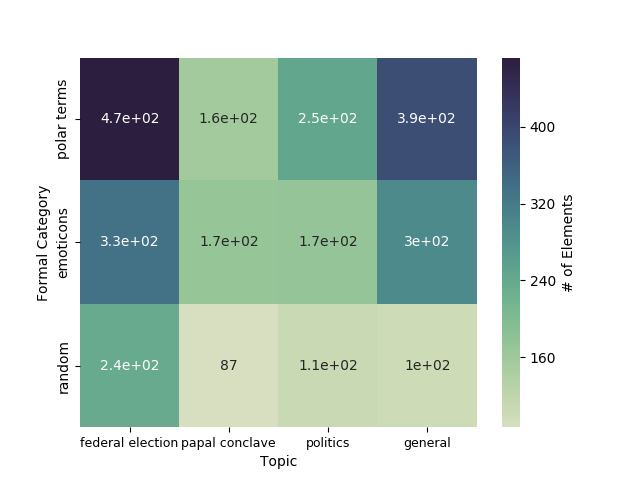
\includegraphics[width=\linewidth]{img/sentiment_stat.png}
  \caption{\texttt{Sentiments}}
\end{subfigure}%
\begin{subfigure}{.5\textwidth}
  \centering
  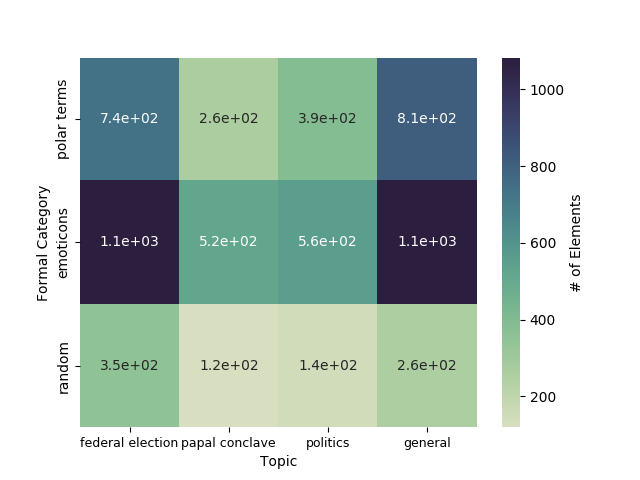
\includegraphics[width=\linewidth]{img/emo-expression_stat.png}
  \caption{\texttt{Emotional expressions}}
\end{subfigure}
}
\caption{Distribution of sentiments and emotional expressions across
  topics and formal categories.}\label{fig:distr}
\end{figure*}

\begin{figure*}[htbp!]
{
\centering
\begin{subfigure}{.5\textwidth}
  \centering
  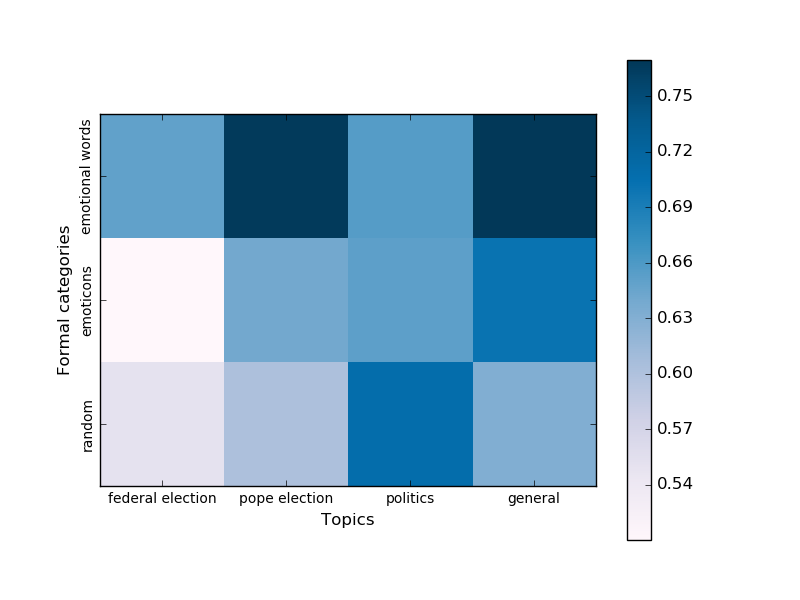
\includegraphics[width=\linewidth]{img/sentiment_agreement.png}
  \caption{\texttt{Sentiments}}
\end{subfigure}%
\begin{subfigure}{.5\textwidth}
  \centering
  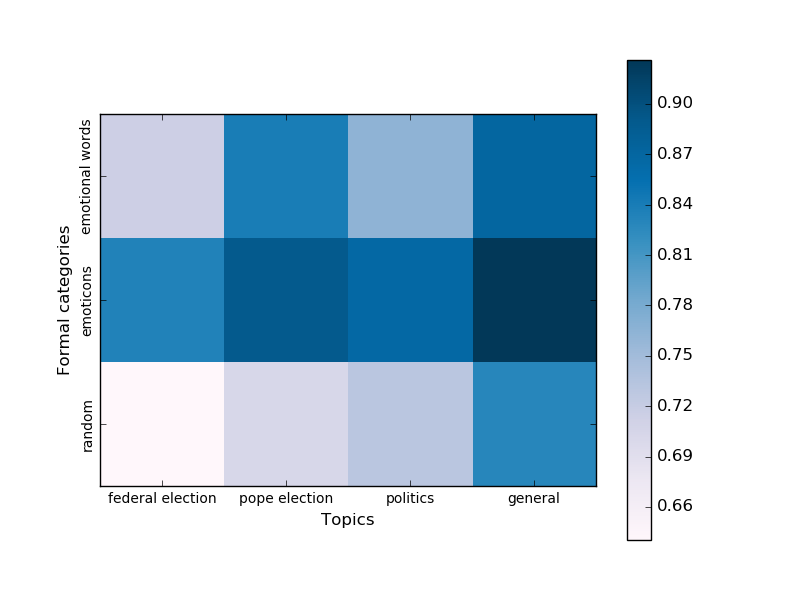
\includegraphics[width=\linewidth]{img/emo-expression_agreement.png}
  \caption{\texttt{Emotional expressions}}
\end{subfigure}
}
\caption{Inter-annotators agreement on sentiments and emotional
  expressions across topics and formal categories.}\label{fig:distr}
\end{figure*}

As can be seen from the scores, reaching a consensus about the
polarities of emotional terms was much easier than agreeing on the
value of this attribute for complete opinions.  Similar to
Example~\ref{example:sent-disagr}, one of the main reasons for these
disagreements were subjective opinions containing smileys, especially
in the cases when the polarity of the emoticon contradicted the
polarity of its preceding sentence, e.g., ``Ich hasse die
Piratenpartei \smiley{}'' (\emph{I hate the Pirate Party {\upshape
    \smiley{}}}).

Finally, to check how the selection criteria that we applied initially
for sampling our corpus affected the final distribution of sentiments
and polar expressions, we generated statistics plots on the
frequencies and agreement level of these elements in the annotated
dataset.  As can be seen from the figures, the stratification
according to topics and formal features has notably influenced both
the number of these elements and the difficulty of their
interpretation.

According to Figure \ref{fig:distr}, federal elections and topically
unfiltered tweets are the ones that contain the major part of the
opinions.  A similar tendency is also observed for emotional
expressions, though, in this case, the formal grouping appears to play
a more important role than topics.  Interestingly enough, the higher
number of polar terms does not necessarily imply a higher number of
targeted sentiments.  We can recognize that from the fact that, even
though most of the polar terms show up in the second row of the plot
(i.e., in microblogs with smileys), the biggest number of opinions
appear in row one (i.e., in tweets containing terms from the SentiWS
lexicon).

Regarding the inter-annotator agreement, we can see that the highest
reliability of annotated opinions is achieved on general tweets taken
from casual everyday conversations.  This group is also the one with
the highest IAA scores for emotional expressions.  A different
situation, however, is observed for these two element types as to the
formal groups of the tweets.  In this case, the first formal category
(i.e., tweets with lexicon terms) appears to comprise messages with
the most reliably annotated sentiments.  For emotional expressions,
however, the emoticons category, again, is the one with the highest
achieved result, whereas, for opinions, the agreement scores in this
row are among the lowest.  This finding suggests that, even though,
smileys are typically recognized as polar entities, the question
whether they relate to something particular in the tweet or rather
express the general mood of the author might often be difficult to
answer.

%% \subsection{Corpus Statistics}\label{subsec:snt:stat}

%% \begin{table}[h]
%%   \centering\small
%%   \caption[Sentiment corpus statistics]{Statistics on the annotated
%%     sentiment corpus.\\ POL = corpus part with discussions about
%%     general politic topics; FE = corpus part describing the federal
%%     election 2013; PE = corpus part with discussions about the Pope
%%     election 2013; GEN = part of the corpus containing tweets with no
%%     particular topic}
%%   \begin{tabular}{|>{\centering}p{0.15\textwidth}|*{4}{>{\centering}p{\oosixthClmnWidth}|}
%%       >{\centering\bfseries}p{\oosixthClmnWidth}|*{4}{>{\centering}p{\oosixthClmnWidth}|}
%%       >{\centering\bfseries}p{\oosixthClmnWidth}|}
%%     \hline

%%     \multirow{2}{*}{\parbox{0.13\textwidth}{\centering Markable Type}}
%%     & \multicolumn{5}{>{\centering}p{7\oosixthClmnWidth}|}{Annotator
%%       1} &
%%     \multicolumn{5}{>{\centering}p{7\oosixthClmnWidth}|}{Annotator
%%       2}\tabularnewline\cline{2-11}

%%     & POL & FE & PE & GEN & Total & POL & FE & PE & GEN &
%%     Total\tabularnewline\hline

%%     Sentiment & 212 & 222 & 163 & 131 & 728 & 317 & 335 & 314 & 305 & 1271
%%     \tabularnewline\hline

%%     Source & 101 & 119 & 68 & 73 & 361 & 114 & 109 & 94 & 85 & 402
%%     \tabularnewline\hline

%%     Target & 229 & 279 & 184 & 151 & 843 & 342 & 369 & 328 & 324 & 1363
%%     \tabularnewline\hline

%%     Emotional Expression & 727 & 689 & 581 & 811 & 2808 & 662 & 669 & 671 & 768 & 2770
%%     \tabularnewline\hline

%%     Intensifier & 16 & 32 & 14 & 44 & 106 & 31 & 35 & 31 & 58 & 155
%%     \tabularnewline\hline

%%     Diminisher & 2 & 4 & 3 & 2 & 11 & 2 & 9 & 4 & 2 & 17
%%     \tabularnewline\hline

%%     Negation & 18 & 15 & 23 & 14 & 70 & 33 & 33 & 31 & 23 & 120
%%     \tabularnewline\hline
%%   \end{tabular}
%%   \label{table:sentiment-agreement-topics}
%% \end{table}


\subsection{Related Work}
\newpage
